\documentclass[11pt,a4paper]{article}
\usepackage[a4paper,margin=2.2cm]{geometry}
\usepackage{fontspec}
\setmainfont{Noto Serif CJK TC}[BoldFont={Noto Serif CJK TC Bold}]
\setsansfont{Noto Sans CJK TC}[BoldFont={Noto Sans CJK TC Bold}]
\XeTeXlinebreaklocale "zh"
\XeTeXlinebreakskip = 0pt plus 1pt
\usepackage{amsmath,amssymb,bm}
\usepackage{tabularx,booktabs,array}
\usepackage{enumitem}
\usepackage[most]{tcolorbox}
\usepackage{xcolor}
\usepackage{graphicx}
\usepackage{hyperref}
\hypersetup{colorlinks=true,linkcolor=blue!50!black}
\setlength{\parindent}{0pt}
\setlength{\parskip}{0.5em}
\renewcommand{\arraystretch}{1.35}

\definecolor{bluebg}{HTML}{F5F8FB}  \definecolor{blueframe}{HTML}{AFC0D2}  \definecolor{bluetitle}{HTML}{1F3864}
\definecolor{greenbg}{HTML}{F3F9F4} \definecolor{greenframe}{HTML}{A8CDB1} \definecolor{greentitle}{HTML}{1E5631}
\definecolor{redbg}{HTML}{FCF4F4}   \definecolor{redframe}{HTML}{DDB1B1}   \definecolor{redtitle}{HTML}{8B1E1E}
\definecolor{amberbg}{HTML}{FCF8EE} \definecolor{amberframe}{HTML}{DCC896} \definecolor{ambertitle}{HTML}{7A5200}
\definecolor{graybg}{HTML}{F6F6F6}  \definecolor{grayframe}{HTML}{C4C4C4}  \definecolor{graytitle}{HTML}{333333}
\newcommand{\boxmark}{\rule[0.02em]{0.62em}{0.62em}}
\tcbset{
  boxblue/.style ={colback=bluebg, colbacktitle=bluebg, colframe=blueframe, coltitle=bluetitle},
  boxgreen/.style={colback=greenbg,colbacktitle=greenbg,colframe=greenframe,coltitle=greentitle},
  boxred/.style  ={colback=redbg,  colbacktitle=redbg,  colframe=redframe,  coltitle=redtitle},
  boxamber/.style={colback=amberbg,colbacktitle=amberbg,colframe=amberframe,coltitle=ambertitle},
  boxgray/.style ={colback=graybg, colbacktitle=graybg, colframe=grayframe, coltitle=graytitle},
  notebox/.style={enhanced,breakable,sharp corners,boxrule=0.6pt,titlerule=0pt,
    fonttitle=\bfseries\large,toptitle=6pt,bottomtitle=2pt,
    left=10pt,right=10pt,top=4pt,bottom=8pt,before skip=10pt,after skip=12pt,
    boxblue}}
\newtcolorbox{cbox}[2][boxblue]{notebox,#1,title={\boxmark\enspace #2}}
\newtcolorbox{takeaway}[1][重點提示]{notebox,boxamber,title={\boxmark\enspace #1}}
\newtcolorbox{derivationbox}[1][完整推導]{notebox,boxblue,title={\boxmark\enspace #1}}
\newtcolorbox{trapbox}[1][常見陷阱]{notebox,boxred,title={\boxmark\enspace #1}}
\newtcolorbox{recipebox}[1][解題流程]{notebox,boxgreen,title={\boxmark\enspace #1}}

% ===== 記號 =====
\newcommand{\Vsq}[1]{\overline{V^2_{n,\text{#1}}}}
\newcommand{\Isq}[1]{\overline{I^2_{n,\text{#1}}}}
\newcommand{\gm}{g_m}
% ===== 例題標示 =====
\definecolor{extag}{HTML}{3A3A3A}
\definecolor{extagbg}{HTML}{E4E4E4}
\newcommand{\extag}[1]{\colorbox{extagbg}{\textcolor{extag}{\sffamily\bfseries\,例 #1\,}}}
\newcommand{\exhead}[3]{\par\medskip\noindent\extag{#1}\enspace{\bfseries #3}\enspace{\small\color{black!55}(p.#2)}\par\nopagebreak\smallskip}
\newcommand{\exref}[1]{\textcolor{extag}{\textbf{\sffamily 例 #1}}}
\newcommand{\rfig}[3]{\begin{center}\includegraphics[width=#2\linewidth]{figs/fig7_#1.png}\\[0.1em]{\small\sffamily 圖 7.#1\quad #3}\end{center}}

\begin{document}
\begin{center}{\LARGE\bfseries\sffamily ECD 單元複習講義：Noise（雜訊）}\\[0.3em]{\large Razavi, \emph{Design of Analog CMOS Integrated Circuits}, Ch.~7（pp.~219--272）}\end{center}

\textbf{記號約定}：本講義沿用課本寫法，$\Vsq{}$、$\Isq{}$ 都代表「每 1\,Hz 頻寬」的雜訊功率譜密度（單位 V$^2$/Hz、A$^2$/Hz），即 $\Delta f=1$\,Hz；要得到總雜訊必須再對頻率積分。$\gamma$ 若無特別說明指\textbf{通道熱雜訊係數}（長通道 $2/3$，經驗上取 $\approx1$），不是 body effect 係數。圖片皆截取自課本，圖說後標註頁碼。課本的 Examples 一律以 \extag{7.x} 標籤開頭、獨立成段，內文提到時以 \exref{7.x} 標示，方便翻閱。

\begin{takeaway}[考試重點地圖]
\begin{enumerate}[leftmargin=2.2em]
  \item \textbf{三個元件模型背到反射}：電阻 $4kTR$（或 $4kT/R$）、MOS 通道熱雜訊 $4kT\gamma g_m$（D–S 電流源）、flicker $\dfrac{K}{C_{ox}WL}\dfrac1f$（串在閘極的電壓源）。
  \item \textbf{input-referred noise 的求法}：短路輸入求 $\Vsq{in}$、開路輸入求 $\Isq{in}$；配合「閘極參考」lemma $\overline{V_n^2}=\overline{I_n^2}/g_m^2$，幾乎所有單級電路都能一行寫出。
  \item \textbf{各拓撲的 $\Vsq{in}$ 公式與直觀}：CS、電流源負載 CS、互補 CS、CG（含 $\Isq{in}=4kT/R_D$）、SF、cascode、差動對（CS 的 2 倍）、5T OTA。訊號路徑上的電晶體要 $g_m$ 大，當電流源的要 $g_m$ 小。
  \item \textbf{積分型題目}：$kT/C$（與 $R$ 無關）、單極點雜訊頻寬 $\frac{\pi}{2}f_p$、flicker 積分得 $\ln(f_H/f_L)$、corner frequency $f_C$、SNR 計算。
  \item \textbf{期中考題範圍}：專題資料夾中的〈Midterm Problems〉收錄了本章習題 7.1--7.7（輸入參考熱雜訊、flicker、分佈閘極電阻 $R_G/3$、lemma 證明）。第 \ref{sec:problems} 節逐題整理解法。
\end{enumerate}
\end{takeaway}

% =====================================================================
\section{雜訊是隨機過程：只能談平均功率與頻譜}

\subsection{平均功率與功率譜密度（PSD）}
雜訊的瞬時值無法預測，但平均功率通常可預測（課本 p.~219--221）。把負載電阻省略、以 V$^2$ 為單位：
\begin{align}
P_{av}=\lim_{T\to\infty}\frac1T\int_{-T/2}^{+T/2}x^2(t)\,dt\qquad[\text{V}^2],\qquad V_{\text{rms}}=\sqrt{P_{av}}
\end{align}
PSD $S_x(f)$ 是「在 $f$ 附近 1\,Hz 頻寬內」的平均功率，單位 V$^2$/Hz；常取根號寫成 nV/$\sqrt{\text{Hz}}$。例如 $3\,\text{nV}/\sqrt{\text{Hz}}$ 只是表示 1\,Hz 頻寬內功率為 $(3\times10^{-9})^2$\,V$^2$。

\exhead{7.1}{221}{聲音頻譜與平均時間}
男聲高頻成分較弱、女聲較強，所以女聲的時域波形變化較快（頻譜告訴我們波形變化有多快）。平均時間 $T$ 要涵蓋最低頻成分的數個週期：語音最低約 20\,Hz，取約 10 個週期，$T\approx500$\,ms。

\textbf{白雜訊}（white noise）：PSD 為常數。嚴格說總功率無限大，所以實際上指「在關心的頻帶內平坦」。

\subsection{線性系統對頻譜的整形：$S_Y=S_X|H|^2$}
若雜訊通過轉移函數 $H(s)$ 的 LTI 系統：
\begin{align}
\boxed{S_Y(f)=S_X(f)\,|H(f)|^2},\qquad H(f)=H(s=j2\pi f)
\end{align}
這是整章最常用的定理：每個雜訊源先求到輸出的轉移函數，平方後乘上自己的 PSD。

\textbf{單邊與雙邊頻譜}：實信號的 $S_x(f)$ 是偶函數，把負頻率部分折到正頻率，得到單邊頻譜（值變 2 倍）。本章所有元件公式（如 $4kTR$）都是\textbf{單邊}，積分範圍 $0\to\infty$。
\rfig{09}{0.6}{(a) 雙邊頻譜，(b) 單邊頻譜（p.224）}

\subsection{相關與不相關雜訊源的疊加}
兩個雜訊相加後的功率：
\begin{align}
P_{av}=P_{av1}+P_{av2}+\lim_{T\to\infty}\frac1T\int 2x_1(t)x_2(t)\,dt
\end{align}
第三項是相關項。不同元件產生的雜訊彼此獨立 $\Rightarrow$ 相關項為零 $\Rightarrow$ \textbf{功率可以疊加}（電壓不能直接相加）。唯一要小心的是：同一個雜訊源經兩條路徑到達同一點（例如差動對中 $I_{n1}$ 同時流過 $R_{D1}$ 與 $R_{D2}$），這時要先把\textbf{電壓}相加再平方。

\subsection{SNR 與雜訊分析四步驟}
$\text{SNR}=P_{sig}/P_{noise}$，弦波振幅 $A$ 時 $P_{sig}=A^2/2$；$P_{noise}=\int S_{noise}(f)\,df$。頻寬開得越寬、積到的雜訊越多，所以\textbf{頻寬應限制在應用所需的最小值}。

\exhead{7.2}{227}{積分白雜訊（數值）}
$S=5\times10^{-16}$\,V$^2$/Hz，1\,MHz 頻寬 $\Rightarrow P=5\times10^{-10}$\,V$^2$，$V_{\text{rms}}=22.4\,\mu$V。注意總雜訊單位是 V$^2$，不是 V$^2$/Hz。

\textbf{分析四步驟}（p.~227）：(1) 找出所有雜訊源並寫下 PSD；(2) 求每個源到輸出的轉移函數（輸入信號設為零）；(3) 用 $S_Y=S_X|H|^2$ 得到各自的輸出頻譜；(4) 不相關者功率相加，最後對頻率積分得總雜訊。

% =====================================================================
\section{熱雜訊：電阻 $4kTR$、MOSFET $4kT\gamma g_m$}

\subsection{電阻熱雜訊與兩種等效模型}
\begin{align}
\overline{V_n^2}=4kTR\ \ (\text{串聯電壓源})\qquad\Longleftrightarrow\qquad \overline{I_n^2}=\frac{4kT}{R}\ \ (\text{並聯電流源})
\end{align}
$k=1.38\times10^{-23}$\,J/K，$T=300$\,K 時 $kT=4.14\times10^{-21}$\,J。50\,$\Omega$ 電阻：$8.28\times10^{-19}$\,V$^2$/Hz，即 $0.91\,\text{nV}/\sqrt{\text{Hz}}$。熱雜訊在約 100\,THz 以內都是白的。雜訊源極性可任意選，但一旦選定，整個分析中要保持一致。

\exhead{7.4}{230}{兩電阻並聯的雜訊}
用電流源模型，功率相加：$\Isq{tot}=4kT(1/R_1+1/R_2)$，故 $\Vsq{tot}=4kT(R_1\parallel R_2)$，即並聯電阻的熱雜訊等於其等效電阻的熱雜訊。

\subsection{RC 電路的總雜訊：$kT/C$}
\rfig{16}{0.62}{電阻雜訊被 RC 低通整形（p.229）}

\exhead{7.3}{228}{RC 低通濾波器的總輸出雜訊（重要新觀察：$kT/C$ 與 $R$ 無關）}
\begin{derivationbox}[完整推導與計算步驟：RC 低通濾波器的總輸出雜訊 $kT/C$]
\begin{enumerate}[leftmargin=2.2em]
  \item \textbf{寫下雜訊源}：$R$ 以串聯電壓源 $V_R$ 表示，$S_v(f)=4kTR$。
  \item \textbf{求轉移函數}：$\dfrac{V_{out}}{V_R}(s)=\dfrac{1}{RCs+1}\ \Rightarrow\ \left|\dfrac{V_{out}}{V_R}(j2\pi f)\right|^2=\dfrac{1}{4\pi^2R^2C^2f^2+1}$
  \item \textbf{輸出頻譜}：$S_{out}(f)=\dfrac{4kTR}{4\pi^2R^2C^2f^2+1}$
  \item \textbf{對 $f$（不是 $\omega$）積分}：令 $u=2\pi RCf$，$df=du/(2\pi RC)$，
  \[P_{n,out}=\int_0^\infty\frac{4kTR\,df}{4\pi^2R^2C^2f^2+1}=\frac{4kTR}{2\pi RC}\int_0^\infty\frac{du}{u^2+1}=\frac{2kT}{\pi C}\Big[\tan^{-1}u\Big]_0^\infty=\frac{2kT}{\pi C}\cdot\frac{\pi}{2}\]
  \[\boxed{P_{n,out}=\frac{kT}{C}}\]
  \item \textbf{數值與直觀}：
  \begin{itemize}[label=\textperiodcentered,leftmargin=1.5em]
    \item $C=1$\,pF、300\,K：$\sqrt{kT/C}=64.3\,\mu\text{V}_{\text{rms}}$。
    \item 與 $R$ 無關：$R$ 變大時單位頻寬雜訊 $\propto R$ 增加，但頻寬 $\propto 1/R$ 減少，兩者抵消。
    \item 要降低 $kT/C$ 只能加大 $C$（或降溫），這是取樣電路、切換電容電路的根本限制。
  \end{itemize}
\end{enumerate}
\end{derivationbox}

\textbf{注意：}積分要對 $f$ 做，因為 PSD 定義是「每 Hz」；若對 $\omega$ 積分要除以 $2\pi$。

\subsection{MOSFET 通道熱雜訊}
飽和區長通道元件的通道熱雜訊可模型化為 D–S 間的電流源：
\begin{align}
\boxed{\overline{I_n^2}=4kT\gamma g_m},\qquad \gamma=\tfrac23\ (\text{長通道}),\ \text{短通道更大，經驗取}\ \gamma\approx1
\end{align}
\exhead{7.5}{231}{單一 MOSFET 能產生的最大雜訊電壓（重要新觀察）}
\rfig{20}{0.28}{單一 MOSFET 能產生的最大輸出雜訊（p.231）}
負載為理想電流源時，輸出只看到 $r_O$，$\Vsq{out}=4kT\gamma g_m r_O^2$，這是單顆電晶體可能產生的最大雜訊電壓。三個觀察：
\begin{enumerate}[leftmargin=2em]
  \item 雜訊電流 $\propto g_m$：當作\textbf{電流源}的電晶體應使 $g_m$ 小。
  \item 求輸出雜訊時輸入設為零，所以同一電路當 CS 或 CG 看，輸出雜訊相同。
  \item $r_O$ 不是實體電阻，\textbf{不產生雜訊}。
\end{enumerate}

\subsection{閘極分佈電阻 $R_G$ 的雜訊}
\rfig{21}{0.62}{(a) MOS 佈局中的端點電阻；(b) 雜訊模型；(c) 分佈式閘極電阻（p.232）}
閘極多晶矽有分佈電阻 $R_G$。靠近接點的單元電晶體只看到一小段電阻的雜訊，遠端則看到大部分，所以等效集總電阻小於 $R_G$；可證明（習題 7.3，推導見第 \ref{sec:problems} 節）
\begin{align}
R_1=\frac{R_G}{3},\qquad \overline{V^2_{n,R_G}}=4kT\,\frac{R_G}{3}
\end{align}
\textbf{佈局改善}（圖 7.22）：兩端都接金屬 $\Rightarrow$ 分佈電阻 $R_G\to R_G/4$；折成 2 根 finger 也是 $R_G/4$。一般來說，\textbf{切成 $N$ 根並聯 finger，分佈電阻降為 $1/N^2$}。
\exhead{7.6}{233}{4 根 finger 的閘極電阻雜訊}
4 根 finger，每根分佈電阻 $R_G/4$、集總 $R_G/12$，四根並聯 $R_G/48$，雜訊 $4kTR_G/48$。
\rfig{22}{0.5}{降低閘極電阻：(a) 兩側接點，(b) folding（p.232）}
\exhead{7.7}{233}{閘極電阻雜訊可忽略的條件（新觀察）}
要使閘極電阻雜訊可忽略，比較 $4kT\frac{R_G}{3}(g_mr_O)^2\ll 4kT\gamma g_m r_O^2$，得
\begin{align}
\boxed{\frac{R_G}{3}\ll\frac{\gamma}{g_m}}
\end{align}
\textbf{注意：}一般元件模型內含熱雜訊與 flicker 雜訊，但\textbf{不含閘極電阻雜訊}，要由設計者自行加入。

% =====================================================================
\section{Flicker（$1/f$）雜訊：與面積成反比、主宰低頻}

\subsection{模型與物理來源}
氧化層–矽介面的 dangling bonds 形成陷阱能階，載子隨機被捕捉、釋放，造成汲極電流的 flicker 雜訊。飽和區中模型化為串在閘極的電壓源：
\begin{align}
\boxed{\overline{V_n^2}=\frac{K}{C_{ox}WL}\cdot\frac1f},\qquad K\sim10^{-25}\ \text{V}^2\text{F}
\end{align}
\begin{itemize}[leftmargin=2em]
  \item 與偏壓電流、溫度（近似）無關；與\textbf{閘極面積 $WL$} 成反比 $\Rightarrow$ 低雜訊應用中元件面積可達數百 $\mu$m$^2$（本質上是雜訊與閘極電容 $WLC_{ox}$ 的取捨）。
  \item \textbf{PMOS 的 $1/f$ 雜訊通常小於 NMOS}：電洞走「埋入式通道」，離介面較遠，受陷阱影響較小。
  \item 換成汲極電流：$\overline{I^2_{n,1/f}}=\dfrac{K}{C_{ox}WL}\dfrac1f\,g_m^2$。
\end{itemize}

\subsection{積分：$\ln(f_H/f_L)$ 與「無限大」的解讀}
\exhead{7.8}{234}{NMOS 電流源在 1\,kHz--1\,MHz 的熱雜訊與 $1/f$ 雜訊}
\begin{align}
\overline{I^2_{n,th,tot}}&=4kT\gamma g_m(10^6-10^3)\approx4kT\gamma g_m\times10^6\ \text{A}^2\\
\overline{I^2_{n,1/f,tot}}&=\frac{Kg_m^2}{C_{ox}WL}\int_{10^3}^{10^6}\frac{df}{f}=\frac{Kg_m^2}{C_{ox}WL}\ln10^3=\frac{6.91\,Kg_m^2}{C_{ox}WL}
\end{align}
$f_L\to0$ 時積分發散，但物理上代表「觀察時間無限長才會看到的極慢變動」，與熱漂移、老化無法區分；而且是對數相依，$f_L$ 從 1\,kHz 改成 100\,Hz，係數只由 6.91 變為 9.21，所以 $f_L$ 選得粗略也無妨。

\subsection{Corner frequency $f_C$}
\rfig{27}{0.36}{$1/f$ 雜訊 corner frequency（p.235）}
令汲極電流中熱雜訊與 $1/f$ 雜訊相等：
\begin{align}
4kT\gamma g_m=\frac{K}{C_{ox}WL}\frac{1}{f_C}g_m^2\quad\Longrightarrow\quad\boxed{f_C=\frac{K}{C_{ox}WL}\cdot\frac{g_m}{4kT\gamma}}
\end{align}
雖然與面積和 $g_m$ 有關，但給定 $L$ 時相依性很弱，奈米製程約在 10--50\,MHz（NMOS 甚至數百 MHz）。

\exhead{7.9}{236}{由 corner frequency 反推 $K$（數值驗算）}
$W/L=100/0.5$、$g_m=1/100\,\Omega$、$f_C=500$\,kHz、$t_{ox}=90$\,\AA（$C_{ox}=3.84\,\text{fF}/\mu\text{m}^2$）、$\gamma=2/3$：
\[K=f_C\,\gamma\,C_{ox}WL\,\frac{4kT}{g_m}=5\times10^5\cdot\tfrac23\cdot(3.84\times10^{-15}\cdot50)\cdot\frac{1.656\times10^{-20}}{10^{-2}}\approx1.06\times10^{-25}\ \text{V}^2\text{F}\]

% =====================================================================
\section{電路中的雜訊表示法：輸出雜訊與輸入參考雜訊}

\subsection{輸出雜訊：以 CS 級為例}
\rfig{29}{0.48}{(a) CS 級；(b) 含雜訊源（p.237）}
\exhead{7.10}{236}{CS 級的總輸出雜訊}
$M_1$ 的熱雜訊與 $1/f$ 雜訊、$R_D$ 的熱雜訊都以電流源表示，全部流過 $R_D$（$\lambda=0$）：
\begin{align}
\Vsq{out}=\left(4kT\gamma g_m+\frac{K}{C_{ox}WL}\frac1f g_m^2+\frac{4kT}{R_D}\right)R_D^2
\end{align}

\subsection{輸入參考雜訊電壓 $\Vsq{in}$}
輸出雜訊會隨後級增益放大，不能公平比較電路（後接無雜訊放大器 $A_1$ 時輸出雜訊變 $A_1^2$ 倍，但輸出 SNR 不變）。因此把所有雜訊等效成輸入端一個源，使輸出雜訊不變：$\Vsq{in}=\Vsq{out}/A_v^2$。
\rfig{31}{0.6}{輸入參考雜訊電壓的定義（p.237）}
\exhead{7.11}{238}{CS 級的輸入參考雜訊電壓}
\begin{align}
\Vsq{in}=\frac{\Vsq{out}}{g_m^2R_D^2}=4kT\frac{\gamma}{g_m}+\frac{K}{C_{ox}WL}\frac1f+\frac{4kT}{g_m^2R_D}
\end{align}
\begin{itemize}[leftmargin=2em]
  \item 第一項相當於串在閘極、阻值 $\gamma/g_m$ 的電阻熱雜訊；第三項相當於阻值 $(g_m^2R_D)^{-1}$ 的電阻。「等效熱雜訊電阻 $R_T$」即指 $\Vsq{in,th}=4kTR_T$。
  \item \textbf{為何 $R_D$ 越大，$\Vsq{in}$ 越小？}$R_D$ 在輸出的雜訊電壓 $\propto\sqrt{R_D}$，增益 $\propto R_D$。
  \item 輸入參考雜訊是\textbf{虛構量}，無法在輸入端量到；但它直接告訴我們電路能偵測多小的輸入信號。
\end{itemize}

\subsection{為何還需要 $\Isq{in}$：有限輸入阻抗的問題}
\rfig{32}{0.75}{(a) 含 $C_{in}$ 的 CS 級；(b) 由有限源阻抗驅動；(c) 只用電壓源會出錯（p.239）}
若只用 $\Vsq{in}$，前級輸出阻抗 $R_1$ 與 $C_{in}$ 分壓，會得 $\Vsq{out}=\dfrac{4kT\gamma g_mR_D^2}{R_1^2C_{in}^2\omega^2+1}$，即 $R_1\to\infty$ 時 $M_1$ 的輸出雜訊消失，這顯然錯誤。解法是同時用串聯電壓源 $\Vsq{in}$ 與並聯電流源 $\Isq{in}$；兩者對任何線性二埠都是\textbf{充分且必要}的表示。

\begin{center}
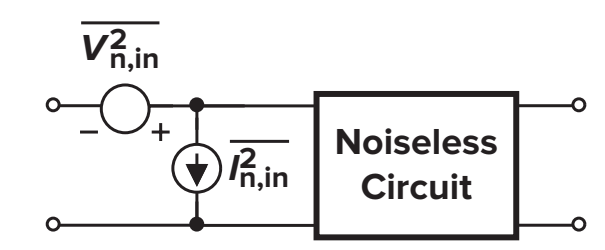
\includegraphics[width=0.27\linewidth]{figs/fig7_33.png}\hspace{1.5em}
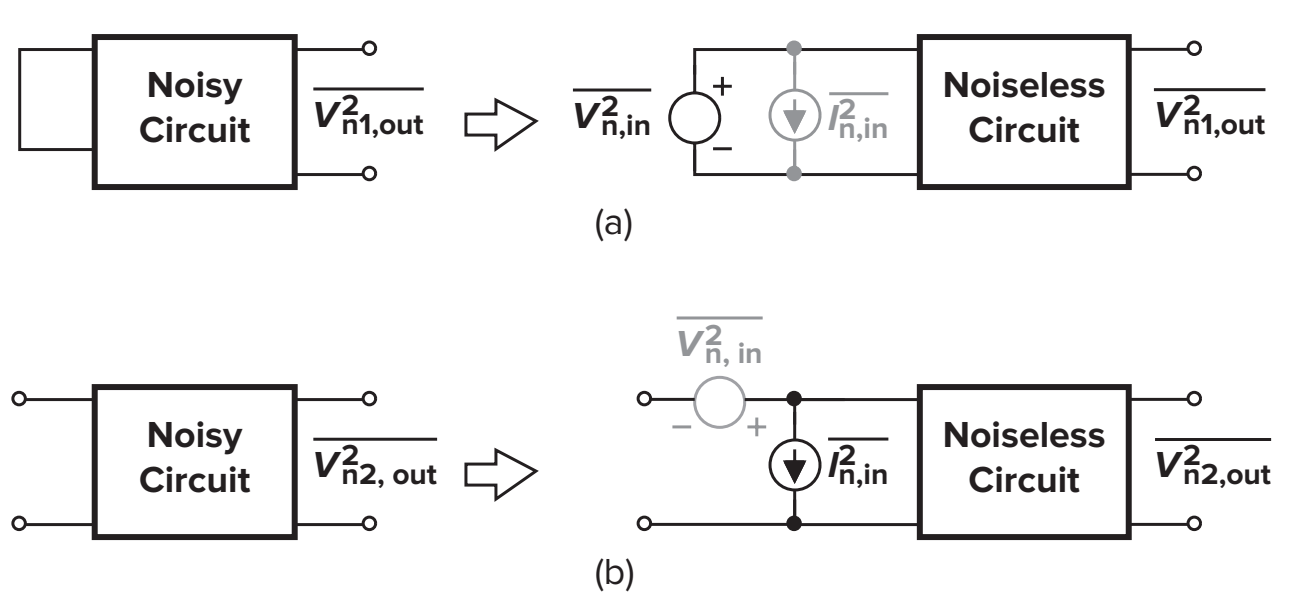
\includegraphics[width=0.52\linewidth]{figs/fig7_34.png}\\[0.1em]
{\small\sffamily 圖 7.33\quad 電壓+電流源表示法（p.239）\qquad 圖 7.34\quad (a) 短路求 $\Vsq{in}$，(b) 開路求 $\Isq{in}$（p.239）}
\end{center}

\textbf{求法（兩個極端源阻抗）}：
\begin{itemize}[leftmargin=2em]
  \item \textbf{輸入短路}（$Z_S=0$）：$\Isq{in}$ 被短路、不影響輸出 $\Rightarrow$ 實際電路的輸出雜訊全來自 $\Vsq{in}$。
  \item \textbf{輸入開路}（$Z_S=\infty$）：$\Vsq{in}$ 沒有電流可推、不影響輸出 $\Rightarrow$ 輸出雜訊全來自 $\Isq{in}$。
\end{itemize}

\exhead{7.12}{239}{CS 級含 $C_{in}$ 的 $\Vsq{in}$ 與 $\Isq{in}$（只考慮熱雜訊）}
\rfig{35}{0.58}{輸入短路與輸入開路（p.240）}
短路時 $\Vsq{in}=4kT\gamma/g_m+4kT/(g_m^2R_D)$。開路時 $\Isq{in}$ 流過 $C_{in}$：
\begin{align}
\Isq{in}\left(\frac{1}{C_{in}\omega}\right)^2g_m^2R_D^2=\left(4kT\gamma g_m+\frac{4kT}{R_D}\right)R_D^2
\ \Rightarrow\ \boxed{\Isq{in}=(C_{in}\omega)^2\frac{4kT}{g_m^2}\left(\gamma g_m+\frac1{R_D}\right)}
\end{align}
低頻時 $\Isq{in}\to0$，所以 MOS 閘極輸入的電路在低頻通常只需考慮 $\Vsq{in}$。

\textbf{何時可忽略 $\Isq{in}$}（圖 7.36）：節點 $X$ 的雜訊 $V_{n,X}=\frac{Z_{in}}{Z_{in}+Z_S}V_{n,in}+\frac{Z_{in}Z_S}{Z_{in}+Z_S}I_{n,in}$，因此
\begin{align}
\boxed{|Z_S|^2\ll\frac{\Vsq{in}}{\Isq{in}}}\ \Rightarrow\ \Isq{in}\ \text{可忽略}
\end{align}
決定 $I_{n,in}$ 重要性的是\textbf{前級的輸出阻抗 $Z_S$}，不是本級的 $Z_{in}$。
\rfig{36}{0.3}{輸入雜訊電流的影響（p.240）}

\textbf{相關性與「不會重複計算」}：$V_{n,in}$ 與 $I_{n,in}$ 常來自同一批雜訊源，彼此高度相關。以圖 7.37 為例，$V_{n,in}=V_{n,M1}+\frac{V_{n,R_D}}{g_mR_D}$、$I_{n,in}=C_{in}s\,V_{n,M1}+\frac{C_{in}s}{g_mR_D}V_{n,R_D}$，用\textbf{電壓疊加}（而非功率）代入節點 $X$，得 $V_{n,X}=V_{n,M1}+V_{n,R_D}/(g_mR_D)$，與 $Z_S$、$C_{in}$ 無關，輸出雜訊與 (7.52) 相同，證明兩源不會重複計算雜訊。

\begin{trapbox}[常見陷阱：輸入參考雜訊的計算]
\begin{enumerate}[leftmargin=2.2em]
  \item \textbf{除以增益平方}：$\Vsq{in}=\Vsq{out}/A_v^2$，不是除以 $A_v$；$\Isq{in}$ 則除以「電流增益」或「轉阻」的平方。
  \item \textbf{$V_{n,in}$ 與 $I_{n,in}$ 相關}：兩者同時作用時（有限 $Z_S$），不可以把功率直接相加，要回到電壓疊加或用附錄 A 的方法。
  \item \textbf{不能對 $\Vsq{in}$ 直接積分}：輸入參考頻譜常是白的（積分發散），總雜訊要在\textbf{輸出}積分後再除以中頻增益平方（第 \ref{sec:bw} 節）。
  \item \textbf{$r_O$ 不產生雜訊}，但會影響轉移函數；題目給 $\lambda\neq0$ 時記得用 $r_O$ 並聯計算輸出阻抗。
\end{enumerate}
\end{trapbox}

\subsection{另一種方法：輸出短路雜訊電流}
有時先求\textbf{輸出短路雜訊電流}較簡單，再乘輸出阻抗得輸出電壓，或除以 $G_m$ 得 $\Vsq{in}$。
\exhead{7.13}{242}{含回授電阻 $R_F$ 的放大器（新電路、新方法：輸出短路電流法）}
\rfig{38}{0.6}{回授電阻 $R_F$ 的放大器（p.242）}
條件：$I_1$ 無雜訊、$\lambda=0$。
\begin{itemize}[leftmargin=2em]
  \item \textbf{求 $\Vsq{in}$}（輸入、輸出都短路，圖 b）：$R_F$ 兩端都是交流地，$\Isq{n1,out}=4kT/R_F+4kT\gamma g_m$。轉導 $G_m=I_{out}/V_{in}=g_m-1/R_F$（圖 c），
  \[\Vsq{in}=\frac{4kT/R_F+4kT\gamma g_m}{(g_m-1/R_F)^2}\]
  \item \textbf{求 $\Isq{in}$}（輸入開路，圖 d）：$V_{n,R_F}$ 直接調變 $V_{GS}$，$\Isq{n2,out}=4kTR_Fg_m^2+4kT\gamma g_m$；電流增益（圖 e）$I_{out}=(g_mR_F-1)I_{in}$，
  \[\Isq{in}=\frac{4kTR_Fg_m^2+4kT\gamma g_m}{(g_mR_F-1)^2}\]
\end{itemize}
此電路輸入短路與開路時的輸出雜訊電壓不同（開路時 $\Vsq{n2,out}=4kT\gamma/g_m+4kTR_F$）。

% =====================================================================
\section{單級放大器的雜訊}

\subsection{Lemma：汲極雜訊電流 $\Leftrightarrow$ 閘極雜訊電壓}
\rfig{39}{0.7}{等效的 CS 級：電流源模型與閘極電壓源模型（p.244）}
\textbf{Lemma}：低頻下，若 $\overline{V_n^2}=\overline{I_n^2}/g_m^2$，則 (a)、(b) 兩電路對\textbf{任意} $Z_S$ 都等效。

\textbf{證明}：兩電路輸出阻抗相同，只需比較輸出短路電流（圖 c、d）。對 (c)：設源極電壓 $V_S$，汲極電流 $I_d=-V_S(g_m+g_{mb}+1/r_O)$，$V_S=Z_S(I_d+I_n)$，輸出短路電流 $I_{out}=I_d+I_n$，解得
\begin{align}
I_{n,out1}=\frac{I_n}{Z_S(g_m+g_{mb}+1/r_O)+1},\qquad I_{n,out2}=\frac{g_mV_n}{Z_S(g_m+g_{mb}+1/r_O)+1}
\end{align}
兩者相等 $\Leftrightarrow V_n=I_n/g_m$。$V_n$ 稱為 $M_1$ 的\textbf{閘極參考雜訊}。
\exhead{7.14}{244}{用 Thevenin 等效證明 lemma}
$Z_L$ 開路時 $Z_S$ 無電流，$V_{Thev1}=I_nr_O$、$V_{Thev2}=g_mV_nr_O$，同樣得 $V_n=I_n/g_m$。

\textbf{用法}：把每顆電晶體的雜訊直接寫成串在閘極的 $4kT\gamma/g_m+K/(C_{ox}WLf)$，再「從那顆電晶體的閘極到輸出的增益」換算，是最快的解題法。（含 $C_{GS}$ 時見習題 7.29。）

\subsection{Common-source 級：電晶體要放大就要 $g_m$ 大}
\begin{align}
\Vsq{in}=4kT\left(\frac{\gamma}{g_m}+\frac{1}{g_m^2R_D}\right)+\frac{K}{C_{ox}WL}\frac1f
\end{align}
電晶體放大閘極電壓信號時 $g_m$ 要最大化；當作定電流源時 $g_m$ 要最小化。

\exhead{7.15}{245}{電流源負載 CS 級的雜訊與 SNR（重要新觀察：$g_{m1}$ 大、$g_{m2}$ 小）}
\rfig{42}{0.5}{電流源負載 CS 級（p.246）}
兩顆電晶體的雜訊電流都流過 $r_{O1}\parallel r_{O2}$：
\begin{align}
\Vsq{out}&=4kT\gamma(g_{m1}+g_{m2})(r_{O1}\parallel r_{O2})^2,\qquad A_v=g_{m1}(r_{O1}\parallel r_{O2})\\
\Vsq{in}&=4kT\gamma\left(\frac{1}{g_{m1}}+\frac{g_{m2}}{g_{m1}^2}\right)
\end{align}
直觀：$g_{m1}$ 增加時輸出雜訊 $\propto\sqrt{g_{m1}}$、增益 $\propto g_{m1}$，所以輸入雜訊下降；$M_2$ 不放大信號，沒有這個好處。

接上負載 $C_L$ 後積分（套用 $kT/C$ 結果）：
\begin{align}
\Vsq{out,tot}=\gamma(g_{m1}+g_{m2})(r_{O1}\parallel r_{O2})\frac{kT}{C_L},\qquad
\text{SNR}_{out}=\frac{C_L}{2\gamma kT}\cdot\frac{g_{m1}^2(r_{O1}\parallel r_{O2})}{g_{m1}+g_{m2}}V_m^2
\end{align}
要提高 SNR 就要加大 $C_L$（縮小頻寬）：寬頻與低雜訊難以兼得。

\exhead{7.16}{247}{互補 CS 級（新電路）}
輸出雜訊同\exref{7.15}，但增益變成 $(g_{m1}+g_{m2})(r_{O1}\parallel r_{O2})$：
\begin{align}
\boxed{\Vsq{in}=\frac{4kT\gamma}{g_{m1}+g_{m2}}}
\end{align}
因為 $M_2$ 也在放大輸入，兩顆的轉導相加，好比並聯。

\textbf{電阻負載 CS 的取捨}：代入 $g_m=2I_D/(V_{GS}-V_{TH})$，
\begin{align}
\Vsq{in}=4kT\left[\frac{\gamma(V_{GS}-V_{TH})}{2I_D}+\frac{(V_{GS}-V_{TH})^2}{4I_D\cdot I_DR_D}\right]
\end{align}
固定壓降 $I_DR_D$ 與 overdrive（$W\propto I_D$）時，增加 $I_D$ 就降低雜訊，代價是功耗。

\exhead{7.17}{247}{電流源負載再並聯 $R_D$ 的 CS 級（含 $1/f$）}
\rfig{44}{0.5}{電流源負載與電阻並聯（p.247）}
$M_2$ 閘極雜訊經增益 $g_{m2}(R_D\parallel r_{O1}\parallel r_{O2})$ 到輸出，再除以主增益 $g_{m1}(R_D\parallel r_{O1}\parallel r_{O2})$：
\begin{align}
\Vsq{in}=4kT\gamma\left(\frac{1}{g_{m1}}+\frac{g_{m2}}{g_{m1}^2}\right)+\frac{1}{C_{ox}f}\left[\frac{K_N}{(WL)_1}+\frac{K_Pg_{m2}^2}{(WL)_2g_{m1}^2}\right]+\frac{4kT}{g_{m1}^2R_D}
\end{align}
$R_D=\infty$ 時退化成\exref{7.15}，$g_{m2}=0$ 時退化成電阻負載 CS。

\textbf{低雜訊 CS 設計方向}：熱雜訊靠提高 $g_{m1}$（$I_D$ 或 $W$，代價為功耗、擺幅、電容）、提高 $R_D$（代價為 headroom、速度）；$1/f$ 雜訊靠加大面積 $WL$（固定 $W/L$ 時 $g_m$ 不變但電容變大）。

\exhead{7.18}{248}{flicker 雜訊電流「與 $W$ 無關」？（觀念陷阱）}
把 $1/f$ 汲極電流寫成 $\frac{K}{WLC_{ox}f}\cdot2\mu_nC_{ox}\frac WL I_D=\frac{2K\mu_nI_D}{L^2f}$ 而得出「與 $W$ 無關」是錯的。公平比較要固定 $I_D$ \textbf{與} overdrive，應寫成 $\frac{K}{WLC_{ox}f}\frac{4I_D^2}{(V_{GS}-V_{TH})^2}$，可見面積越大雜訊越小。

\exhead{7.19}{248}{電阻負載 CS 級的雜訊設計（設計題）}
\rfig{45}{0.5}{CS 級的總雜訊設計（p.249）}
規格為總輸入參考雜訊 $100\,\mu\text{V}_{\text{rms}}$、功耗 1\,mW、頻寬 1\,GHz（由 $R_D$ 與 $C_L$ 決定）、$V_{DD}=1$\,V。輸出雜訊與積分：
\begin{align}
\Vsq{out}&=(1+\gamma g_mR_D)\frac{4kTR_D}{R_D^2C_L^2\omega^2+1}\ \Rightarrow\ \Vsq{out,tot}=(1+\gamma g_mR_D)\frac{kT}{C_L}\\
\Vsq{in,tot}&=\frac{1+\gamma g_mR_D}{g_m^2R_D^2}\cdot\frac{kT}{C_L}=\frac{1+\gamma g_mR_D}{g_m^2R_D}\cdot2\pi kT\cdot\underbrace{\frac{1}{2\pi R_DC_L}}_{1\,\text{GHz}}=(100\,\mu\text{V})^2\\
&\Rightarrow\ \frac1{g_m}\left(\frac{1}{g_mR_D}+\gamma\right)=\frac{(100\,\mu\text{V})^2}{2\pi kT\times1\,\text{GHz}}=384\,\Omega
\end{align}
取 $g_mR_D=3$、$\gamma=1$：$1/g_m=288\,\Omega$、$R_D=864\,\Omega$；$I_D=1$\,mA 時 $I_DR_D=864$\,mV，只剩 $V_{DS}=136$\,mV，擺幅很小（可試 $g_mR_D=2$ 或 4 比較 headroom）。

\subsection{Common-gate 級：負載雜訊直接成為輸入雜訊電流}
\begin{center}
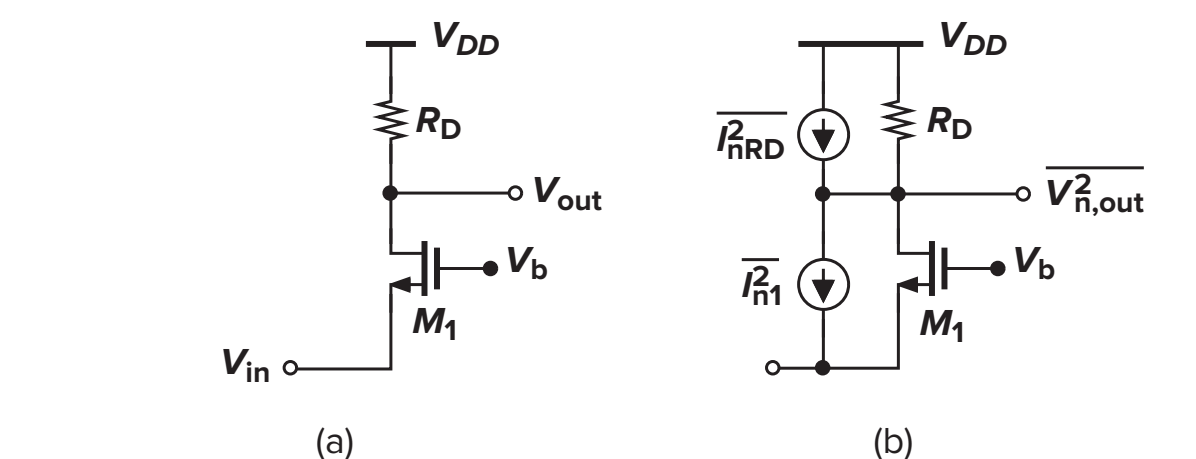
\includegraphics[width=0.36\linewidth]{figs/fig7_46.png}\hspace{1em}
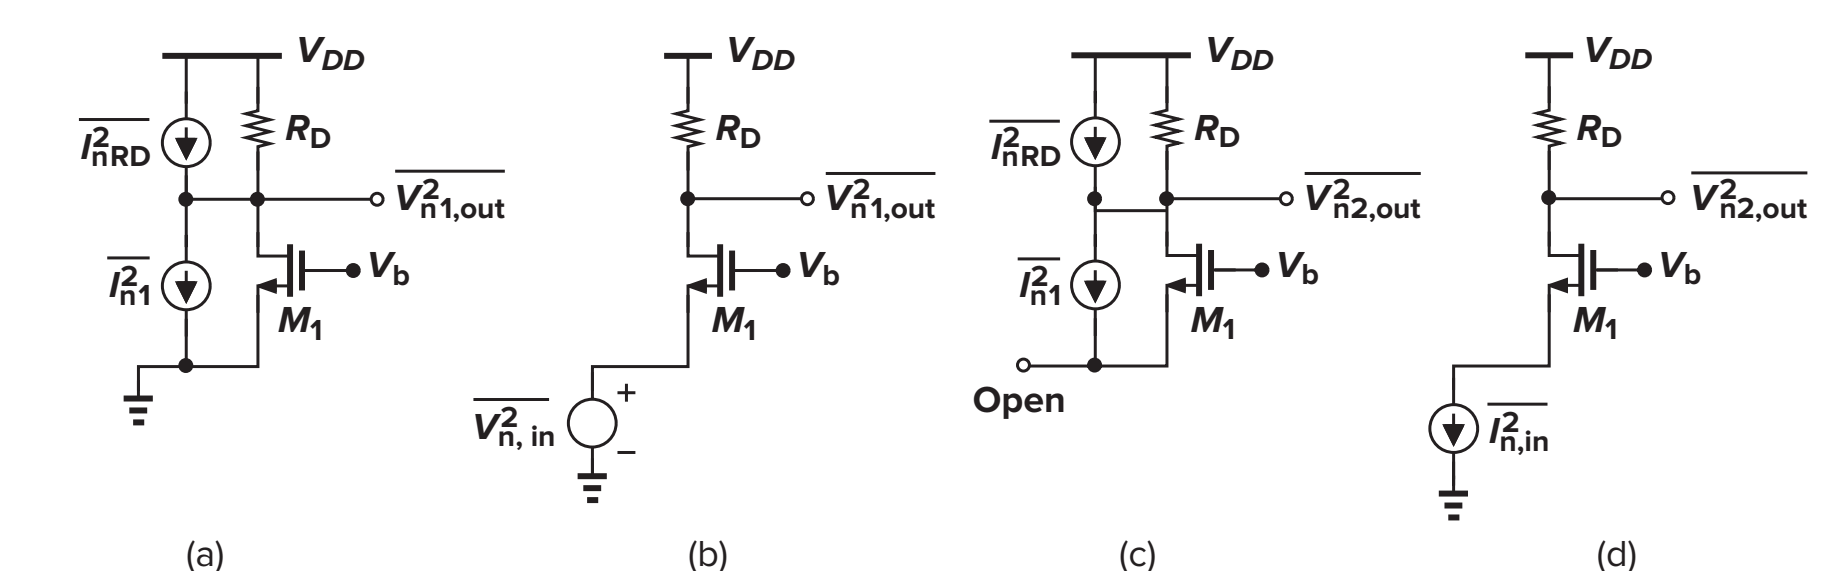
\includegraphics[width=0.56\linewidth]{figs/fig7_47.png}\\[0.1em]
{\small\sffamily 圖 7.46\quad CG 級與雜訊源\qquad 圖 7.47\quad (a)(b) 短路求 $\Vsq{in}$；(c)(d) 開路求 $\Isq{in}$（p.250）}
\end{center}
CG 輸入阻抗低，\textbf{即使低頻 $\Isq{in}$ 也不可忽略}。
\begin{itemize}[leftmargin=2em]
  \item \textbf{輸入短路}：$\left(4kT\gamma g_m+\frac{4kT}{R_D}\right)R_D^2=\Vsq{in}(g_m+g_{mb})^2R_D^2$
  \[\Vsq{in}=\frac{4kT(\gamma g_m+1/R_D)}{(g_m+g_{mb})^2}\]
  \item \textbf{輸入開路}：源極節點 KCL 給 $I_{n1}+I_{D1}=0$，$M_1$ 自己的雜訊電流在內部循環，對輸出\textbf{沒有貢獻}；輸出雜訊只剩 $4kTR_D$，
  \[\boxed{\Isq{in}=\frac{4kT}{R_D}}\]
\end{itemize}
\textbf{缺點}：CG 沒有電流增益，負載的雜訊電流被原封不動地參考回輸入。

\rfig{48}{0.3}{偏壓電流源 $M_2$ 的雜訊（p.251）}
\textbf{偏壓電流源的雜訊}（圖 7.48）：輸入短路時 $M_2$ 的雜訊電流不流過 $R_D$，對 $\Vsq{in}$ 無貢獻；輸入開路時全部流經 $M_1$、$R_D$，所以 $\overline{I^2_{n2}}$ \textbf{直接加到 $\Isq{in}$}。要讓 $g_{m2}$ 小，但 $g_{m2}=2I_{D2}/(V_{GS2}-V_{TH2})$，給定電流時需大 overdrive，會吃掉 $V_b$ 與輸出擺幅。

\exhead{7.20}{251}{PMOS 電流源負載的 CG 級（新電路）}
\rfig{49}{0.3}{PMOS 電流源負載的 CG 級（p.251）}
全部電晶體飽和：
\begin{align}
\Vsq{in}=4kT\gamma\frac{g_{m1}+g_{m3}}{(g_{m1}+g_{mb1})^2},\qquad
\Isq{in}=4kT\gamma(g_{m2}+g_{m3})
\end{align}
（$M_3$ 的雜訊電流參考到輸入時，在 $g_mr_O\gg1$ 下 $I_{n,in}|_{M3}\approx I_{n3}$。）兩者都正比於\textbf{電流源}電晶體的 $g_m$。

\textbf{CG 的 $1/f$ 雜訊}（圖 7.50，各管 $1/f$ 雜訊以閘極電壓源表示）：
\begin{align}
\Vsq{in}=\frac{1}{C_{ox}f}\left[\frac{g_{m1}^2K_N}{(WL)_1}+\frac{g_{m3}^2K_P}{(WL)_3}\right]\frac{1}{(g_{m1}+g_{mb1})^2},\qquad
\Isq{in}=\frac{1}{C_{ox}f}\left[\frac{g_{m2}^2K_N}{(WL)_2}+\frac{g_{m3}^2K_P}{(WL)_3}\right]
\end{align}
分別加到上面的熱雜訊結果即為總雜訊。

\subsection{Source follower：增益小於 1 卻加雜訊}
\rfig{51}{0.45}{(a) Source follower；(b) 含雜訊源（p.253）}
輸入阻抗高，通常忽略 $\Isq{in}$。$M_2$ 的雜訊電流看到 $\frac1{g_{m1}}\parallel\frac1{g_{mb1}}\parallel r_{O1}\parallel r_{O2}$，除以 $A_v^2$ 後：
\begin{align}
\Vsq{in}=\overline{V^2_{n1}}+\frac{\Vsq{out}|_{M2}}{A_v^2}=4kT\gamma\left(\frac1{g_{m1}}+\frac{g_{m2}}{g_{m1}^2}\right)
\end{align}
形式與電流源負載 CS 相同。由於只會加雜訊而增益 $<1$，低雜訊放大鏈中盡量避免 SF。

\subsection{Cascode 級：低頻時 cascode 管幾乎不貢獻}
\rfig{52}{0.5}{(a) Cascode；(b)(c) $M_2$ 的雜訊模型（p.254）}
低頻下 $M_1$、$R_D$ 的貢獻與 CS 相同：$\Vsq{in}=4kT\left(\frac{\gamma}{g_{m1}}+\frac{1}{g_{m1}^2R_D}\right)$。$M_2$：若忽略 $M_1$ 的 $\lambda$，$I_{n2}+I_{D2}=0$，對輸出無貢獻；換成閘極電壓源看，節點 $X$ 阻抗很大，$V_{n2}$ 到輸出增益很小（就像源極退化很大的 CS）。

\textbf{高頻}：$X$ 點電容 $C_X$ 使 $\frac{V_{n,out}}{V_{n2}}\approx\frac{-R_D}{1/g_{m2}+1/(C_Xs)}$ 上升，同時 $C_X$ 分流 $M_1$ 的信號電流、降低主增益，所以 cascode 的輸入參考雜訊在高頻可能明顯惡化。

% =====================================================================
\section{電流鏡的雜訊：二極體接法元件的 $1/f$ 雜訊會被放大 $N$ 倍}
\rfig{53}{0.72}{(a) 以 $C_B$ 抑制 $M_{REF}$ 雜訊的電流鏡；(b) 小訊號模型；(c) 等效電路（p.255）}
$(W/L)_1=N(W/L)_{REF}$。$M_{REF}$ 與其雜訊的 Thevenin 等效：開路電壓 $V_{n,REF}$（因 $I_{REF}$ 為理想電流源，$V_1$ 必為 0），內阻 $1/g_{m,REF}$。與 $C_B$ 成低通後和 $V_{n1}$ 一起驅動 $M_1$：
\begin{align}
\Isq{out}=\left(\frac{g_{m,REF}^2}{C_B^2\omega^2+g_{m,REF}^2}\overline{V^2_{n,REF}}+\overline{V^2_{n1}}\right)g_{m1}^2
\end{align}
同 $L$ 時面積比為 $N$，$\overline{V^2_{n,REF}}=N\overline{V^2_{n1}}$，故
\begin{align}
\Isq{out}=\left(\frac{N\,g_{m,REF}^2}{C_B^2\omega^2+g_{m,REF}^2}+1\right)g_{m1}^2\overline{V^2_{n1}},\qquad
\text{可忽略條件：}\ \boxed{C_B^2\gg\frac{(N-1)g_{m,REF}^2}{\omega^2}}
\end{align}
數值（課本）：$N=5$、$g_{m,REF}=1/(200\,\Omega)$、最低頻 1\,MHz $\Rightarrow C_B\gg1.59$\,nF；要十倍抑制需 5.03\,nF，晶片上不切實際。

\rfig{54}{0.5}{(a) 在閘極串 $R_B$ 降低截止頻率；(b) 以 MOS $M_R$ 實現大電阻（p.256）}
\textbf{改善}：串入 $R_B$，截止頻率降為 $[(1/g_{m,REF}+R_B)C_B]^{-1}$，
\begin{align}
\Isq{out}=\left[\frac{g_{m,REF}^2}{(1+g_{m,REF}R_B)^2C_B^2\omega^2+g_{m,REF}^2}\left(\overline{V^2_{n,REF}}+\overline{V^2_{n,R_B}}\right)+\overline{V^2_{n1}}\right]g_{m1}^2
\end{align}
$R_B$ 本身有熱雜訊，但在其熱雜訊接近 $M_{REF}$ 的 $1/f$ 雜訊之前可以做得很大；上限由 $R_B$ 與 $C_B$ 的面積取捨決定（以及閘極漏電流造成的 dc 誤差）。實作上用小 overdrive 的 MOS $M_R$（窄長），$M_C$ 寬短。

% =====================================================================
\section{差動對的雜訊：輸入參考雜訊功率是 CS 的 2 倍}

\subsection{電阻負載差動對}
\rfig{56}{0.55}{差動對輸入參考雜訊的計算（p.257）}
低頻時 $\Isq{in}$ 可忽略。$I_{n1}$ 與 $I_{n2}$ 不相關，$P$ 點\textbf{不是}虛接地，不能用半電路，只能逐一計算。由圖 (c)(d)，$I_{n1}$ 一半流經 $R_{D1}$、一半流經 $M_2$ 與 $R_{D2}$（同源、相關，電壓直接相加）：
\begin{align}
V_{n,out}|_{M1}&=\frac{I_{n1}}{2}R_{D1}+\frac{I_{n1}}{2}R_{D2}\ \xrightarrow{R_{D1}=R_{D2}=R_D}\ \Vsq{out}|_{M1}=\overline{I^2_{n1}}R_D^2\\
\Vsq{out}&=\left(\overline{I^2_{n1}}+\overline{I^2_{n2}}\right)R_D^2+2(4kTR_D)=8kT(\gamma g_mR_D^2+R_D)\\
\Vsq{in}&=\frac{\Vsq{out}}{g_m^2R_D^2}=\boxed{8kT\left(\frac{\gamma}{g_m}+\frac{1}{g_m^2R_D}\right)}
\end{align}
\rfig{57}{0.36}{用 lemma：每管雜訊串在閘極（p.258）}
用 lemma 更快：兩管各串 $4kT\gamma/g_m$，$R_{D1}$、$R_{D2}$ 的雜訊各除以 $g_m^2R_D^2$，直接得到上式。加入 $1/f$：
\begin{align}
\Vsq{in,tot}=8kT\left(\frac{\gamma}{g_m}+\frac{1}{g_m^2R_D}\right)+\frac{2K}{C_{ox}WL}\frac1f
\end{align}
\textbf{結論}：每管 $g_m$ 相同時，差動對的輸入參考雜訊電壓是 CS 的 $\sqrt2$ 倍（訊號路徑上元件數加倍）；且同尺寸下功耗也是 2 倍。一般而言，\textbf{全差動電路的 $\Vsq{in}$ = 半電路的 2 倍}。

\textbf{尾電流雜訊}：輸入差動為零且完全對稱時，$I_{SS}$ 雜訊平分到兩邊，只產生共模雜訊。偏離平衡時 $\Delta I_{D1}-\Delta I_{D2}\approx g_{m0}\left(1+\frac{I_n}{2I_{SS}}\right)\Delta V_{in}$，雜訊調變轉導而產生少量差動雜訊，通常可忽略。

\exhead{7.21}{259}{差動對做成浮接大電阻（新電路）}
次臨界偏壓的差動對可做成 $\approx2/g_{m1}$ 的浮接電阻，其雜訊：$\overline{V^2_{n,AB}}=8kT\gamma(g_{m1}+g_{m3})\frac1{g_{m1}^2}+\frac{2K}{(WL)_1C_{ox}f}+\frac{2K}{(WL)_3C_{ox}f}\left(\frac{g_{m3}}{g_{m1}}\right)^2$，比同值歐姆電阻更吵，也更不線性。

\subsection{電流源負載差動對}
\exhead{7.22}{260}{電流源負載差動對的輸入參考雜訊（新電路、新方法）}
\rfig{59}{0.5}{(a) 電流源負載差動對；(b) 雜訊源；(c) $M_3$ 雜訊電流的分流（p.260）}
$M_1$、$M_2$ 的雜訊已是輸入串聯源，只需把 $M_3$、$M_4$ 參考到輸入。$M_3$ 的雜訊電流分流到 $r_{O3}$ 與看入 $M_1$ 汲極的 $R_X=r_{O4}+2r_{O1}$：
\begin{align}
I_{nA}=g_{m3}V_{n3}\frac{r_{O4}+2r_{O1}}{2r_{O4}+2r_{O1}},\qquad I_{nB}=g_{m3}V_{n3}\frac{r_{O3}}{2r_{O4}+2r_{O1}}
\end{align}
$V_{nXY}=V_{nX}-V_{nY}=g_{m3}V_{n3}\dfrac{r_{O3}r_{O1}}{r_{O3}+r_{O1}}$，即 $M_3$ 的雜訊電流乘上 $r_{O1}\parallel r_{O3}$（也可用把 $V_{n3}$ 拆成兩個差動分量再用半電路驗證）。$M_4$ 同理，功率相加後除以 $g_{m1}^2(r_{O1}\parallel r_{O3})^2$：
\begin{align}
\Vsq{in}=2\overline{V^2_{n1}}+2\frac{g_{m3}^2}{g_{m1}^2}\overline{V^2_{n3}}
=8kT\gamma\left(\frac1{g_{m1}}+\frac{g_{m3}}{g_{m1}^2}\right)+\frac{2K_N}{C_{ox}(WL)_1f}+\frac{2K_P}{C_{ox}(WL)_3f}\frac{g_{m3}^2}{g_{m1}^2}
\end{align}

\subsection{五電晶體 OTA}
\begin{center}
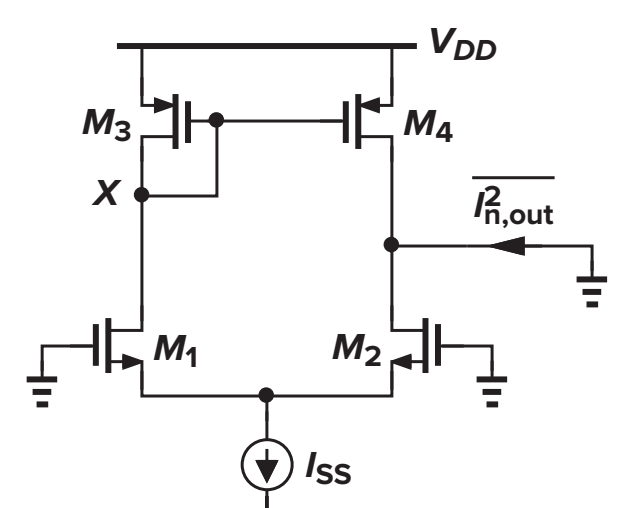
\includegraphics[width=0.28\linewidth]{figs/fig7_61.png}\hspace{2em}
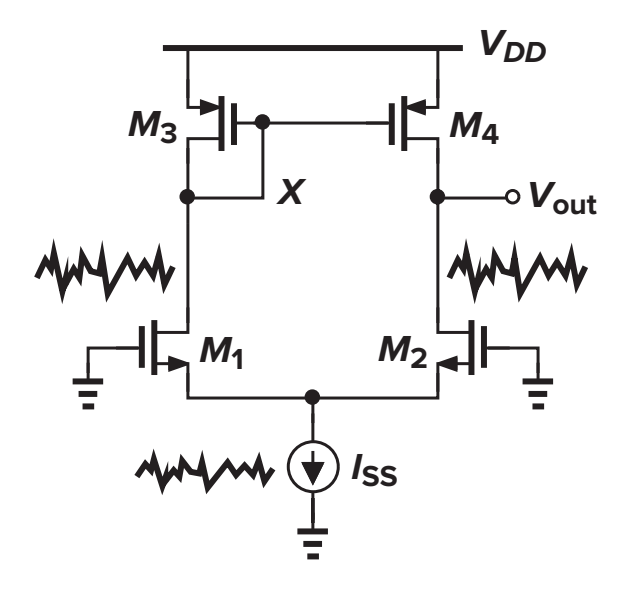
\includegraphics[width=0.24\linewidth]{figs/fig7_62.png}\\[0.1em]
{\small\sffamily 圖 7.61\quad 輸出短路雜訊電流\qquad 圖 7.62\quad 尾電流雜訊的影響（p.262）}
\end{center}
因不對稱，改求 Norton 等效（輸出短路電流）。OTA 的 $G_m\approx g_{m1,2}$：
\begin{itemize}[leftmargin=2em]
  \item $M_1$、$M_2$：$g_{m1,2}^2(4kT\gamma/g_{m1}+4kT\gamma/g_{m2})$。
  \item $M_3$：雜訊電流 $4kT\gamma g_{m3}$ 主要流過二極體阻抗 $1/g_{m3}$，在 $M_4$ 閘極產生 $4kT\gamma/g_{m3}$，再乘 $g_{m4}^2$ 出現在輸出；$M_4$ 自己的雜訊直接流入短路。
\end{itemize}
\begin{align}
\Isq{out}=4kT\gamma(2g_{m1,2}+2g_{m3,4}),\qquad
\Vsq{in}=\frac{\Isq{out}R_{out}^2}{G_m^2R_{out}^2}=8kT\gamma\left(\frac1{g_{m1,2}}+\frac{g_{m3,4}}{g_{m1,2}^2}\right)
\end{align}
與全差動電路相同。差別在\textbf{尾電流雜訊}：OTA 輸出等於 $V_X$，$I_{SS}$ 雜訊平分後在 $X$ 產生 $\overline{I_n^2}/(4g_{m3}^2)$，直接出現在輸出（全差動電路則只是共模）。

% =====================================================================
\section{雜訊–功耗取捨、雜訊頻寬與輸入雜訊積分}\label{sec:bw}

\subsection{線性縮放：雜訊功率減半需付出兩倍功耗}
\rfig{63}{0.55}{(a) 以縮放降低雜訊；(b) 等效為兩電路並聯；(c) 佈局觀點（p.263）}
把 $W/L$ 與 $I_D$ 加倍、$R_D$ 減半：增益與擺幅不變，$g_m$ 與閘極面積都加倍，\textbf{輸入參考熱雜訊與 $1/f$ 雜訊功率都正好減半}（$-3$\,dB），代價是功耗（與輸入電容）加倍。等同兩個原電路並聯：兩個不相關 Thevenin 雜訊源經分壓各剩 $1/2$，
\begin{align}
\Vsq{out}=\frac{\overline{V^2_{n1,out}}}{4}+\frac{\overline{V^2_{n2,out}}}{4}=\frac{\overline{V^2_{n1,out}}}{2}
\end{align}
輸入開路時可證 $\Isq{in}$ 加倍（兩份並聯電流源相加）。這個取捨的前提是頻寬由應用決定、保持不變，且 $\Isq{in}$ 可忽略。

\subsection{雜訊頻寬 $B_n$}
\rfig{65}{0.58}{(a) 多極點輸出雜訊頻譜；(b) 雜訊頻寬的概念（p.264）}
定義 $B_n$ 使 $V_0^2\cdot B_n=\int_0^\infty\Vsq{out}\,df$，其中 $V_0^2$ 為低頻雜訊。可公平比較低頻雜訊相同、高頻轉移函數不同的電路。\textbf{單極點系統}：
\begin{align}
B_n=\int_0^\infty\frac{df}{1+(f/f_p)^2}=f_p\Big[\tan^{-1}(f/f_p)\Big]_0^\infty=\boxed{\frac{\pi}{2}f_p}
\end{align}
（$kT/C$ 其實就是 $4kTR\cdot\frac{\pi}{2}\cdot\frac{1}{2\pi RC}$。）

\subsection{不能在輸入端積分}
\rfig{66}{0.6}{輸入參考頻譜為白雜訊，積分發散（p.265）}
CS 級（只看 $M_1$ 熱雜訊）的輸入參考頻譜就是 $4kT\gamma/g_m$，對頻率積分為無限大；而輸出頻譜被 $C_L$ 低通，可積分得 $\gamma g_mR_D\,kT/C_L$。正確做法：\textbf{在輸出積分，再除以低頻（中頻）增益平方}：
\begin{align}
\Vsq{in,tot}=\gamma g_mR_D\frac{kT}{C_L}\cdot\frac{1}{g_m^2R_D^2}=\frac{\gamma}{g_mR_D}\cdot\frac{kT}{C_L}
\end{align}

\subsection{附錄 A：避開 $V_{n,in}$、$I_{n,in}$ 相關性的方法}
若電路的輸出雜訊幾乎不隨源阻抗 $Z_S$（短路到開路）改變（例如 $C_{GD}$ 可忽略的 CS：$\overline{V^2_{n1,out}}=\overline{V^2_{n2,out}}=4kT\gamma g_mR_D^2+4kTR_D$），則 $\Isq{in}=\Vsq{in}/|Z_{in}|^2$，$I_{n,in}=V_{n,in}/Z_{in}$ 百分之百相關，代入後節點 $X$ 恆有 $V_{n,X}=V_{n,in}$。因此可\textbf{拿掉 $I_{n,in}$，只要用 $Z_{in}$ 負載前級}即可。若此條件不成立，就把前後級視為同一個電路一起求 $V_{n,in}$、$I_{n,in}$（圖 7.69）。

% =====================================================================
\section{總比較表：各拓撲的輸入參考熱雜訊}
以下皆為低頻、每 Hz 的熱雜訊；$1/f$ 雜訊把每顆電晶體的 $4kT\gamma/g_m$ 換成 $K/(C_{ox}WLf)$，並乘上相同的增益比例即可。

\begin{tabularx}{\linewidth}{>{\raggedright}p{2.3cm}>{\raggedright}p{5.0cm}>{\raggedright}p{2.6cm}X}
\toprule
電路 & $\Vsq{in}$ & $\Isq{in}$ & 重點與直觀\tabularnewline\midrule
CS，電阻負載 & $4kT\left(\frac{\gamma}{g_m}+\frac{1}{g_m^2R_D}\right)$ & $(C_{in}\omega)^2\frac{4kT}{g_m^2}\,\times$ $(\gamma g_m+\frac1{R_D})$；低頻 $\approx0$ & 提高 $g_m$、$R_D$ 降雜訊；代價為功耗、headroom\tabularnewline
CS，電流源負載 & $4kT\gamma\left(\frac1{g_{m1}}+\frac{g_{m2}}{g_{m1}^2}\right)$ & $\approx0$ & 負載管 $g_{m2}$ 要小（大 overdrive）\tabularnewline
互補 CS & $\dfrac{4kT\gamma}{g_{m1}+g_{m2}}$ & $\approx0$ & 兩管都在放大，轉導相加\tabularnewline
CG（$R_D$ 負載） & $\dfrac{4kT(\gamma g_m+1/R_D)}{(g_m+g_{mb})^2}$ & $\dfrac{4kT}{R_D}$（$+4kT\gamma g_{m2}$ 偏壓管） & 低頻 $\Isq{in}$ 不可忽略；$M_1$ 不貢獻 $\Isq{in}$\tabularnewline
CG（\exref{7.20}） & $4kT\gamma\dfrac{g_{m1}+g_{m3}}{(g_{m1}+g_{mb1})^2}$ & $4kT\gamma\,\times$ $(g_{m2}+g_{m3})$ & 都正比於電流源管的 $g_m$\tabularnewline
Source follower & $4kT\gamma\left(\frac1{g_{m1}}+\frac{g_{m2}}{g_{m1}^2}\right)$ & 可忽略 & 增益 $<1$ 又加雜訊，低雜訊鏈避免\tabularnewline
Cascode & 低頻同 CS（$M_2$ 可忽略） & $\approx0$ & 高頻 $C_X$ 使 $M_2$ 雜訊上升\tabularnewline
差動對，電阻負載 & $8kT\left(\frac{\gamma}{g_m}+\frac{1}{g_m^2R_D}\right)$ & $\approx0$ & CS 的 2 倍（功率）；尾電流只產生共模\tabularnewline
差動對，電流源負載 / 5T OTA & $8kT\gamma\left(\frac1{g_{m1}}+\frac{g_{m3}}{g_{m1}^2}\right)$ & $\approx0$ & 兩者相同；OTA 的尾電流雜訊會出現在輸出\tabularnewline
\bottomrule
\end{tabularx}

% =====================================================================
\section{題型與期中考題解法}\label{sec:problems}

本節的題號對應課本習題，也就是〈Midterm Problems〉中的第 7 章題目（7.1--7.7）。題目若無特別說明，使用課本 Table 2.1 參數：$\mu_nC_{ox}=134.4\,\mu$A/V$^2$（$\mu_n=350\,\text{cm}^2/\text{V·s}$、$C_{ox}=3.84\,\text{fF}/\mu\text{m}^2$）、$V_{DD}=3$\,V、全部飽和。以下數值取 $kT=4.14\times10^{-21}$\,J、$\gamma=2/3$（長通道；若老師要求 $\gamma=1$ 則照比例修改）。

\begin{trapbox}[常見陷阱：習題中「$\lambda=\gamma=0$」的 $\gamma$ 是 body effect]
習題 7.6--7.9 寫「Assume that $\lambda=\gamma=0$」，這裡的 $\gamma$ 是 \textbf{body effect 係數}（即 $g_{mb}=0$），不是通道熱雜訊係數。電晶體的熱雜訊 $4kT\gamma g_m$ \textbf{仍然存在}，不可以把它也設成零，否則電晶體就沒有雜訊了。
\end{trapbox}

\subsection{題型一：求 input-referred thermal noise voltage}
\textbf{辨識特徵}：「Calculate the input-referred thermal noise voltage」，MOS 閘極輸入。\\
\textbf{步驟}：(1) 每顆電晶體用 lemma 寫成閘極串聯源 $4kT\gamma/g_m$，電阻寫成 $4kTR$ 或 $4kT/R$；(2) 求每個源到輸出的增益（或對輸出短路電流的轉導）；(3) 除以主輸入到輸出的增益平方，功率相加。

\textbf{習題 7.1}（CS，$W/L=50/0.5$、$I_D=1$\,mA、$R_D=2$\,k$\Omega$，100\,MHz 頻寬的總輸入參考熱雜訊）：
\begin{align}
g_m&=\sqrt{2\mu_nC_{ox}\tfrac WLI_D}=\sqrt{2(134.4\,\mu)(100)(1\,\text{m})}=5.18\,\text{mS}\\
\Vsq{in}&=4kT\left(\frac{\gamma}{g_m}+\frac{1}{g_m^2R_D}\right)=1.656\times10^{-20}\,(128.6+18.6)=2.44\times10^{-18}\ \text{V}^2/\text{Hz}\\
V_{n,in,tot}&=\sqrt{2.44\times10^{-18}\times10^8}\approx\boxed{15.6\,\mu\text{V}_{\text{rms}}}\quad(\gamma=1\ \text{時約}\ 18.7\,\mu\text{V}_{\text{rms}})
\end{align}
（題目直接問「輸入參考雜訊在 100\,MHz 頻寬內」，故把白頻譜乘以頻寬；這與第 \ref{sec:bw} 節「在輸出積分」不矛盾，因為此處已明確給定頻寬。）

\rfig{71}{0.55}{習題 7.6 的六個電路（p.268）}
\textbf{習題 7.6}（$\lambda=0$、$g_{mb}=0$）：
\begin{itemize}[leftmargin=2em]
  \item \textbf{(a) 源極退化 CS}：$R_S$ 的雜訊電壓串在源極，等效於串在閘極；$R_D$ 的雜訊電流用 $G_m=g_m/(1+g_mR_S)$ 參考回去：
  \[\Vsq{in}=\frac{4kT\gamma}{g_m}+4kTR_S+\frac{4kT(1+g_mR_S)^2}{g_m^2R_D}\]
  \item \textbf{(b) Source follower，$R_S$ 負載}：輸出短路時 $G_m=g_m$，$R_S$ 的雜訊電流 $4kT/R_S$ 直接是輸出短路電流：
  \[\Vsq{in}=\frac{4kT\gamma}{g_m}+\frac{4kT}{g_m^2R_S}\]
  \item \textbf{(d) 二極體接法負載 + 源極退化}：負載雜訊電流 $4kT\gamma g_{m2}$，同樣用 $G_m=g_{m1}/(1+g_{m1}R_S)$：
  \[\Vsq{in}=\frac{4kT\gamma}{g_{m1}}+4kTR_S+\frac{4kT\gamma g_{m2}(1+g_{m1}R_S)^2}{g_{m1}^2}\]
  \item \textbf{(c)(e)(f)}：含回授電阻 $R_F$ 的電路，建議用「輸出短路雜訊電流 $\div G_m^2$」法（同\exref{7.13}）：先短路輸出求每個源的短路電流與 $G_m$，避免處理 $R_F$ 兩端的負載效應。
\end{itemize}

\subsection{題型二：設計／取捨（給定雜訊比例求尺寸或擺幅）}
\textbf{習題 7.2}（圖 7.42，$(W/L)_1=50/0.5$、$I_{D1}=I_{D2}=0.1$\,mA、$V_{DD}=3$\,V；$M_2$ 對輸入參考雜訊\textbf{電壓}（非平方）的貢獻為 $M_1$ 的 $1/5$，求最大輸出擺幅）：
\begin{align}
\sqrt{\frac{4kT\gamma g_{m2}/g_{m1}^2}{4kT\gamma/g_{m1}}}=\sqrt{\frac{g_{m2}}{g_{m1}}}=\frac15\ \Rightarrow\ g_{m2}=\frac{g_{m1}}{25}
\end{align}
$g_{m1}=\sqrt{2(134.4\,\mu)(100)(0.1\,\text{m})}=1.64$\,mS，$V_{ov1}=2I_D/g_{m1}=0.122$\,V；$g_{m2}=65.6\,\mu$S，$|V_{ov2}|=2I_D/g_{m2}=3.05$\,V。\\
擺幅 $=V_{DD}-V_{ov1}-|V_{ov2}|<0$：\textbf{以題目數據，此規格不可行}（要求 $M_2$ 的 overdrive 超過 $V_{DD}$）。若把條件理解為「雜訊功率比 $1/5$」，則 $g_{m2}=g_{m1}/5$、$|V_{ov2}|=0.61$\,V，最大擺幅 $\approx3-0.122-0.61=2.27$\,V。作答時建議兩種都寫並說明，展現你理解「電流源管 $g_m$ 小 $\leftrightarrow$ overdrive 大 $\leftrightarrow$ 擺幅小」的取捨。

\subsection{題型三：flicker noise}
\textbf{習題 7.5}（圖 7.70，互補 CS：$V_{in}$ 同時接 $M_1$、$M_2$ 閘極）：
\rfig{70}{0.17}{習題 7.5（p.268）}
兩管的 $1/f$ 閘極源各經自己的 $g_m(r_{O1}\parallel r_{O2})$ 到輸出，主增益 $(g_{m1}+g_{m2})(r_{O1}\parallel r_{O2})$：
\begin{align}
\Vsq{in,1/f}=\frac{1}{C_{ox}f}\cdot\frac{g_{m1}^2\frac{K_N}{(WL)_1}+g_{m2}^2\frac{K_P}{(WL)_2}}{(g_{m1}+g_{m2})^2}
\end{align}
\textbf{其他 flicker 題}：corner frequency 用 $f_C=\frac{K}{C_{ox}WL}\frac{g_m}{4kT\gamma}$；頻帶積分得 $\ln(f_H/f_L)$；電流鏡要注意 $N$ 倍放大（第 6 節）。

\subsection{題型四：證明題}
\textbf{習題 7.4}（證明 (7.73)）：見第 5.1 節 lemma 的證明，關鍵是寫出 $V_S=Z_S(I_d+I_n)$、$I_d=-V_S(g_m+g_{mb}+1/r_O)$ 兩式後消去 $V_S$。

\begin{cbox}[boxgray]{補充：習題 7.3 分佈閘極電阻等效為 $R_G/3$ 的證明}
把閘極切成 $n$ 段，每段電阻 $R_G/n$、雜訊電壓 $V_k$（彼此不相關，$\overline{V_k^2}=4kTR_G/n$），每段配一個單元電晶體 $g_{mu}=g_m/n$。忽略通道雜訊、閘極電流為零，則第 $j$ 個單元的閘極電壓是它與接點之間所有段雜訊之和 $\sum_{k\le j}V_k$。
\begin{enumerate}[leftmargin=2.2em]
  \item \textbf{總汲極雜訊電流}：$I_d=g_{mu}\sum_{j=1}^n\sum_{k=1}^jV_k=g_{mu}\sum_{k=1}^n(n-k+1)V_k$，同一個 $V_k$ 影響 $n-k+1$ 個單元（這些是相關的，要先相加電壓）。
  \item \textbf{取功率}（不同 $k$ 不相關）：$\overline{I_d^2}=g_{mu}^2\sum_{m=1}^nm^2\cdot\frac{4kTR_G}{n}\approx\frac{g_m^2}{n^2}\cdot\frac{n^3}{3}\cdot\frac{4kTR_G}{n}=g_m^2\cdot4kT\frac{R_G}{3}$
  \item \textbf{結論}：等效於閘極串一個 $\boxed{R_G/3}$ 的集總電阻。
\end{enumerate}
\end{cbox}

\subsection{題型五：總積分雜訊與 SNR}
\textbf{辨識特徵}：給 $C_L$ 或頻寬，問 total／rms noise 或 SNR。\\
\textbf{步驟}：寫出輸出頻譜（通常是白頻譜乘單極點）$\to$ 用 $\int_0^\infty\frac{4kTR\,df}{1+(2\pi RCf)^2}=\frac{kT}{C}$ 或 $B_n=\frac{\pi}{2}f_p$ 積分 $\to$ 需要輸入參考時再除以中頻增益平方。代表例：\exref{7.15}、\exref{7.19}，習題 7.15、7.32。

\begin{recipebox}[解題流程總整理]
\begin{enumerate}[leftmargin=2.2em]
  \item \textbf{列雜訊源}：電阻 $4kTR$／$4kT/R$；MOS 熱雜訊 $4kT\gamma g_m$（或閘極 $4kT\gamma/g_m$）；flicker $K/(C_{ox}WLf)$（閘極）；$r_O$ 不產生雜訊。
  \item \textbf{求 $\Vsq{in}$}：輸入短路；每個源到輸出的增益平方 $\div$ 主增益平方，功率相加。有回授電阻或不對稱時改用「輸出短路電流 $\div G_m^2$」。
  \item \textbf{求 $\Isq{in}$}：輸入開路；輸出雜訊 $\div$（轉阻）$^2$。MOS 閘極輸入、低頻時 $\approx0$；CG 一定要算（$4kT/R_D$ + 偏壓管）。
  \item \textbf{同源相關、異源不相關}：同一個源經多條路徑時先加電壓；差動對 $P$ 點不是虛接地。
  \item \textbf{積分}：在輸出積分（$kT/C$、$\frac{\pi}{2}f_p$、$\ln(f_H/f_L)$），再除以中頻增益平方；不要對白的輸入參考頻譜積分。
  \item \textbf{檢查直觀}：訊號路徑管 $g_m\uparrow$ 雜訊 $\downarrow$；電流源管 $g_m\downarrow$ 雜訊 $\downarrow$；差動 = 2 倍 CS；線性縮放 2 倍功耗換 $-3$\,dB。
\end{enumerate}
\end{recipebox}

\end{document}
